% Created 2017-04-26 Wed 16:57
% Intended LaTeX compiler: pdflatex
\documentclass[12pt]{article}
\usepackage[utf8]{inputenc}
\usepackage[T1]{fontenc}
\usepackage{graphicx}
\usepackage{grffile}
\usepackage{longtable}
\usepackage{wrapfig}
\usepackage{rotating}
\usepackage[normalem]{ulem}
\usepackage{amsmath}
\usepackage{textcomp}
\usepackage{amssymb}
\usepackage{capt-of}
\usepackage{hyperref}
\usepackage{indentfirst}
\linespread{1.5}
\author{James Nhan, Matt Koenig, Zackery Lovisa, Thien Le}
\date{\textit{<2017-02-24 Fri>}}
\title{Augmented Escape}
\hypersetup{
 pdfauthor={James Nhan, Matt Koenig, Zackery Lovisa, Thien Le},
 pdftitle={Augmented Escape},
 pdfkeywords={},
 pdfsubject={},
 pdfcreator={Emacs 25.1.1 (Org mode 9.0.3)}, 
 pdflang={English}}
\begin{document}

\maketitle
\begin{align*}
   &\textbf{Target Platform}&&\text{: Microsoft HoloLens} \\
   &\textbf{Target Age}&&\text{: 13+} \\
   &\textbf{Target Rating}&&\text{: T}
\end{align*}

\pagebreak

\tableofcontents

\pagebreak

\section{Story}
\label{sec:org29fb24c}
A mysterious group known only as \emph{The Company} is behind a major conspiracy that will lead to world domination, and you know too much about them. You are being hunted, but death is not your destiny. \emph{The Company} believes anyone can be convinced to join them, and you're no different. They've captured and brough you to a remote location to teach compliance. You will be subjected to various forms of brainwashing and torture techniques. Will you succumb to \emph{The Company}'s will, or will you dash their plans and take them out from inside?

\section{Characters}
\label{sec:org43cc283}
\subsubsection{Axshun Jaxxon}
\label{sec:org4630ebe}
\begin{center}
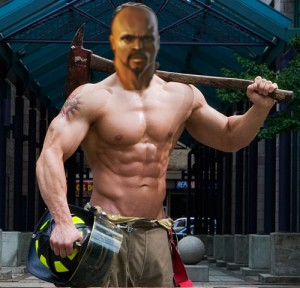
\includegraphics[width=8cm]{./img/axshun-jaxxon.png}
\captionof{figure}{\label{fig:org28ffd04}
Axshun Jaxxon}
\end{center}

\begin{enumerate}
\item Personality
\label{sec:orga194dd2}
Axshun Jaxxon is a rash individual. He is the Leroy Jenkins of Augmented Escape. He uses brute force and brawn over brains. He leaps before he looks. He also loves fried chicken. He may not always get the job done, but at least he's got chicken.

\item Appearance
\label{sec:orgffc86d3}
He has big muscles. He stands 6'6", weighs 280 pounds, is bald, has a goatee, and has one metal pauldron over his right shoulder. The pauldron has a dragon embossment on it. He has tan skin from farming all day. He has no shirt. He has firefighter pants with one leg burnt off at the knee. He wears combat boots.

\item Backstory
\label{sec:org44a4c5a}
He is a firefighter that farms chickens in his free time because he likes chicken. Axshun Jaxxon receives a call from Bearsford, South Dakota dispatch. He is sent on a rescue mission. After rescuing the baby chicks in the farm house, he is alerted to the presence of a child. The child is trapped in the farm house loft. The fire burns so hot and brightly, that his firefighter pants catch flame, resulting in the scorch makes on his left pantleg. A wooden beam from the farm house falls onto his head. He is knocked out cold. Ten days later, he awakes in a sick and twisted game of escaping \emph{The Company}.
\end{enumerate}

\subsubsection{Ben Benson}
\label{sec:org4b5c6f7}
\begin{center}
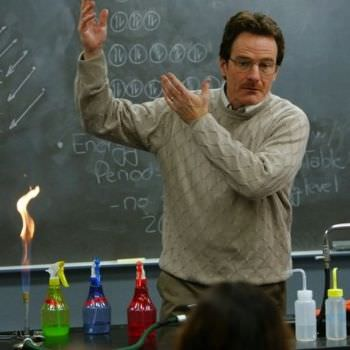
\includegraphics[width=8cm]{./img/ben-benson.png}
\captionof{figure}{\label{fig:org520b481}
Ben Benson}
\end{center}

\begin{enumerate}
\item Personality
\label{sec:org8e35d2a}
Ben Beson is an extremely conservative man born in the secluded areas of Louisiana. He is reserved and quiet. He is cool and calculating. However, when pushed beyond his limits, he is prone to extremely violent outbursts. Whenever possible, Ben Benson will use subterfuge to defeat his enemies. He is the exact opposite of Axshun Jaxxon.

\item Appearance
\label{sec:orgd3d19b8}
He is a mature, white man that wears button up shirts with sweaters. He near sighted and wears glasses. Fluffy brown hair. He is 5'4" and weighs 120 pounds and has no athletic abilities.

\item Backstory
\label{sec:org875260a}
Ben Benson is a Chemistry teacher by trade. In his spare time, he enjoys working at the local car wash. One day, he gets into an argument with his wife, Skylar, over pizza toppings. He gets so angry, he takes their pizza and throws it outside. It lands on their neighbor's house. The next day, a student accidentally mixes the wrong chemicals during the lab and creates mustard gas. This results in an explosion that knocks Ben Benson out. He is taken to the nurse's office. It just so happens that the nurse is an agent of \emph{The Company}. She takes this chance to abduct the genius Chemistry teacher. He wakes up caught in a web of deception and lies. Can he escape the room?
\end{enumerate}

\subsubsection{Yoki Warrior}
\label{sec:org3d69833}

\begin{center}

\includegraphics[width=8cm]{./img/yoki-warrior.png}
\captionof{figure}{\label{fig:org183fc15}
Yoki Warrior}
\end{center}

\begin{enumerate}
\item Personality
\label{sec:org48038ea}
She is a detective, curious by nature. She is a lone with a serious attitude. She can be insenstive to others' plights. She clean, thorough, detailed oriented, and perfectionist. She has depression because of the extinction of her tribe and the disappearance of her lover. Despite her perfectionst attitude, she despises cyborg technology. She especially hates cyborg technology, as she sees it as an abomination and imperfect.

\item Appearance
\label{sec:org9ea383e}
She has light brown skin and long silky hair She wears traditional Native American clothing. Her hair is black and her eyes are also black. As a young woman, she stands 5'3" and weighs 97 pounds. Due to her cyborg reconstruction, her left arm is made of titanium steel alloys. She has an implanted left eye that can perceive ultraviolet and infrared light.

\item Backstory
\label{sec:orgb59be7e}
After single combat with a cyborg bear, she falls unconscious from her grievous wounds. Her noble fighting garnered the attention of the omnipresent \emph{Company}. This prompted them to abduct her into their program. Due to her body being mangled beyond recognition, \emph{The Company} invested \$4 million dollars to rebuild her as cyborg. She is now the thing she hates most: a cyborg.
\end{enumerate}

\subsubsection{World Powers}
\label{sec:org603e0f1}
\begin{center}
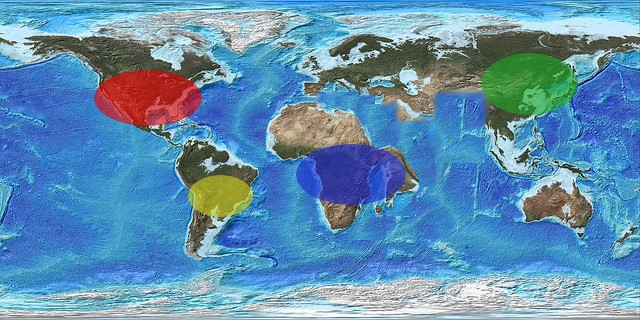
\includegraphics[width=10cm]{./img/world.jpg}
\captionof{figure}{\label{fig:org50920c9}
World Power Distribution.}
\end{center}

\begin{enumerate}
\item The Company
\label{sec:org6b5aa5f}

\begin{center}

\includegraphics[width=4cm]{./img/the-company.png}
\captionof{figure}{\label{fig:org2abebc0}
The Company.}
\end{center}

\begin{enumerate}
\item Backstory
\label{sec:orga31bddc}
In 2018, World War III broke out. Nuclear war raged on for 15 years, destroying the vast majority of the planet and decimating the population to the hundreds of thousands. In the aftermath, a reconstructed, cyborg President Nixon gathered the remnants of the Illuminati and the Free Masons. The resulting merger is \emph{The Company}. Biding their time, they gathered influence over the years. Now, in the year 2142, \emph{The Company} has complete anonymous control over the American world government, granting them free reign over North America.

\item Goals
\label{sec:orgca64453}
\emph{The Company} currently olds captive the continent of North America. Their ultimate goal is to overthrow the other two remaining world governments: China, and the Afindican Warlords as well as the rogue rebels in Antarctica: The Nomads.

\item Influence and Power
\label{sec:org98e43cb}
Having complete anonymous control over North America gives them access to unlimited natural resources (but not rare metals). Using their cyborg technology, they have implanted control chips into the newest generation, giving them access to the largest standing army still in existence today. They utilize \emph{The Program} to recruite the best of the best of the previous generation, such as Axshun Jaxxon, Ben Benson, and Yoki Warrior.
\end{enumerate}

\item Afindican Warlords
\label{sec:orgedf3eb8}

\begin{enumerate}
\item Backstory
\label{sec:org9555611}
The remnants of the India and Africa have merged into one super-continent. They are the result of the tectonic plate shift after the Araibian Plate was nuked from orbit and sunk into the Earth, the massive heat from the Mantle fused the Indian and African tectonic plates into one massive plate that drifted into the center of the Atlantic Ocean. The result is Afindica. Then, the various warlords in the African tribes banded together to create the Afindican Warlords. The new country is the last place on Earth with natural resources. They are rich in Uranium, Cadmium, and other transition metals. They also have the last chicken farm in the world.

\item Goals
\label{sec:org194a8e7}
Being the combination of Africans and Indians, they are a highly spiritual people that want to live simple and separate lives from the rest of the world. They simply want to be left alone.

\item Influence and Power
\label{sec:org9205f0f}
Seeing as Afindica holds the only chickens and rare metals in the world, they have a strong monopoly on the world economy. The other world powers vie for the favor of the Afrindican Warlords. Thus, while they have little military might, they have total economic control.
\end{enumerate}

\item The Chinese Conglomerate
\label{sec:orge016c65}

\begin{enumerate}
\item Backstory
\label{sec:org492792c}
Similar to The Company, the Chinese Conglomerate has complete control of the surviving Asian peoples since 2142. Their main activities are bargaining with the Afindian Warlords and engineering robot armies and workers. Because of the destruction of their homeland and the death of the planet, the Chinese Conglomerate seeks to explore a new home on the Moon.

\item Goals
\label{sec:orgc9122bd}
The Chinese Conglomerate just wants to leave Earth. There is nothing left for the Asian people. The Moon is the only solace from the desolace of Earth.

\item Influence and Power
\label{sec:orgfb2c61a}
The Chinese Conglomerate has the world's largest cyborg army. This makes them the country with the strongest military might and scientific technology.
\end{enumerate}

\item The Nomads
\label{sec:orgd6fa49d}

\begin{enumerate}
\item Backstory
\label{sec:org0def5a9}
The Nomads are a rebellion which started in the wake of The Company's rise to power. They wage war on The Company and are the only group in the world that know of their plans. The Nomads commonly use guerilla tactics and subterfuge to slow down The Company's progression. They fly an orange flag with an white phoenix emblem stitched into the center which symbolizes the rebirth of the Earth's civilization and the burning passion of the people who form The Nomads. The Nomads are based in South America, a piece of land untouched by nuclear war. They use stolen stealth boats and ancient drug-smuggling submarines to reach the shores of North America unnoticed; then, they use repurposed retina scanners to identify people who work at The Company.

\item Goals
\label{sec:org726b9e0}
The Nomads want to strike back at The Company for instigating the devastating nuclear war. The Nomads are made up of the group of survivors that were ravaged by The Company. Their sole driving force is to dismantle The Company in pure revenge.

\item Influence and Power
\label{sec:org0433446}
Being a relatively small and rogue operation, The Nomads have little political influence, yet they retain massive through knowledge and stealth. While not being able to connect politically with the other world powers, they still are able to conduct trade and avoid the wrath of The Company.
\end{enumerate}
\end{enumerate}

\subsubsection{Mittens}
\label{sec:orgafc36a2}
\begin{center}
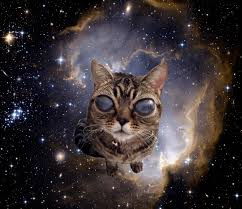
\includegraphics[width=8cm]{./img/mittens.png}
\captionof{figure}{\label{fig:orgc2796f1}
Mittens, the Alien Cat.}
\end{center}

\begin{enumerate}
\item Backstory
\label{sec:orgdfbd59e}
Mittens is an alien cat that was experimented on in Area 51 under The Company's orders. During an attack on Area 51 by the Nomads, he was released and now resides in the Rocky Mountains. Whenever he gets wind of an abduction by The Company, Mittens will use his telepathic powers to communicate with the abductees to assist them in escaping the clutches of The Company.

\item Goals
\label{sec:orgd105c75}
Mittens wants revenge on The Company for ordering the gruesome imprisonment and the painful torture experiments. His only goal is to destroy The Company. Without his people, he is weak. He aims to take down The Company by empowering The Nomads.

\item Influence and Power
\label{sec:orga63da94}
Because Mittens is a secret alien, not many know of his existence. Only those in the Nomad council know of Mittens because the Area 51 staff were all killed in The Nomad attack. Still, Mittens has great power, despite his weak influence. He has alien telekinetic and telepathic abilities.
\end{enumerate}

\section{Core Gameplay}
\label{sec:org7f26ec5}
\begin{center}

\includegraphics[width=8cm]{./img/game-flow.png}
\captionof{figure}{\label{fig:org6a73578}
The game state flow chart.}
\end{center}

\begin{center}
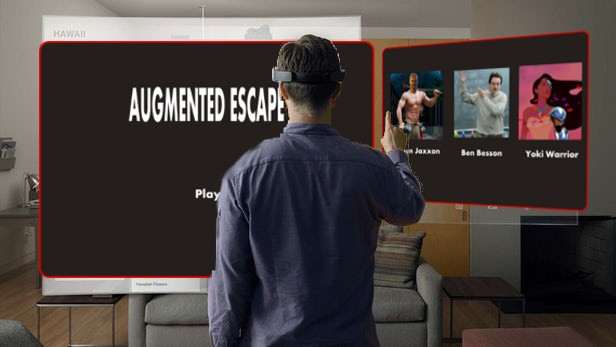
\includegraphics[width=8cm]{./img/main-menu-1.jpg}
\captionof{figure}{\label{fig:orgf17de7c}
Main Menu}
\end{center}

\subsection{Mechanics}
\label{sec:org332f5b8}
\subsubsection{Menu System}
\label{sec:org7d806ed}
Upon loading the application, the player will be greeted with the start menu shown in Figure \ref{fig:org3d740b3}. There will be a play button that the player can choose to start playing and a quit button. Then, the player will be shown a character select menu as shown in Figure \ref{fig:orgcb50883}. On this screen, the player can choose one of three characters: Axshun Jaxxon, Ben Benson, or Yoki Warrior.

\begin{center}
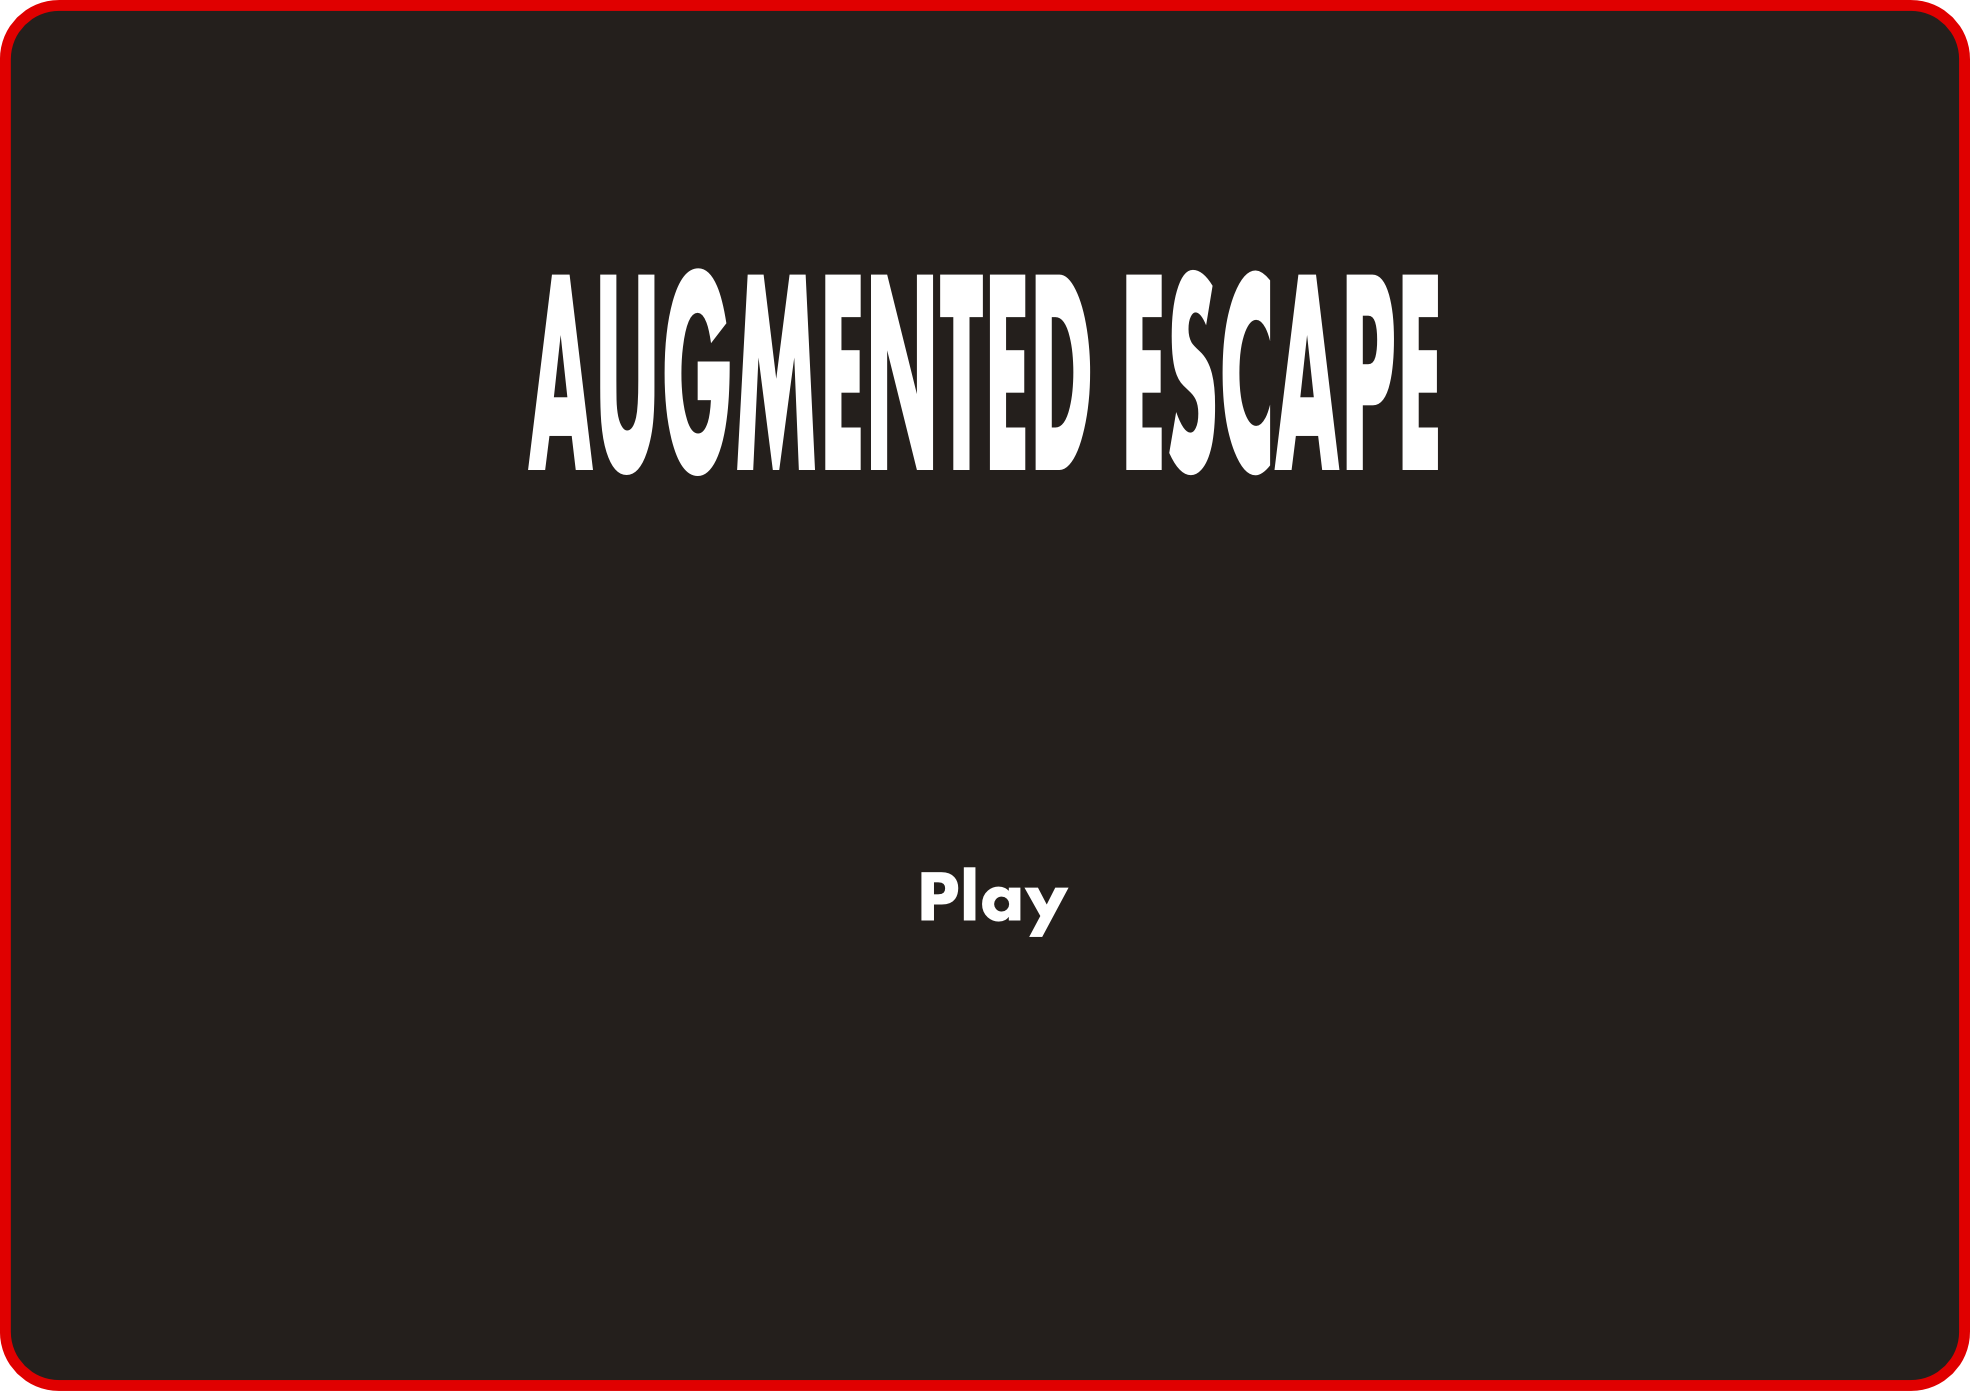
\includegraphics[width=8cm]{./img/start-screen.png}
\captionof{figure}{\label{fig:org3d740b3}
Start Menu}
\end{center}

\begin{center}
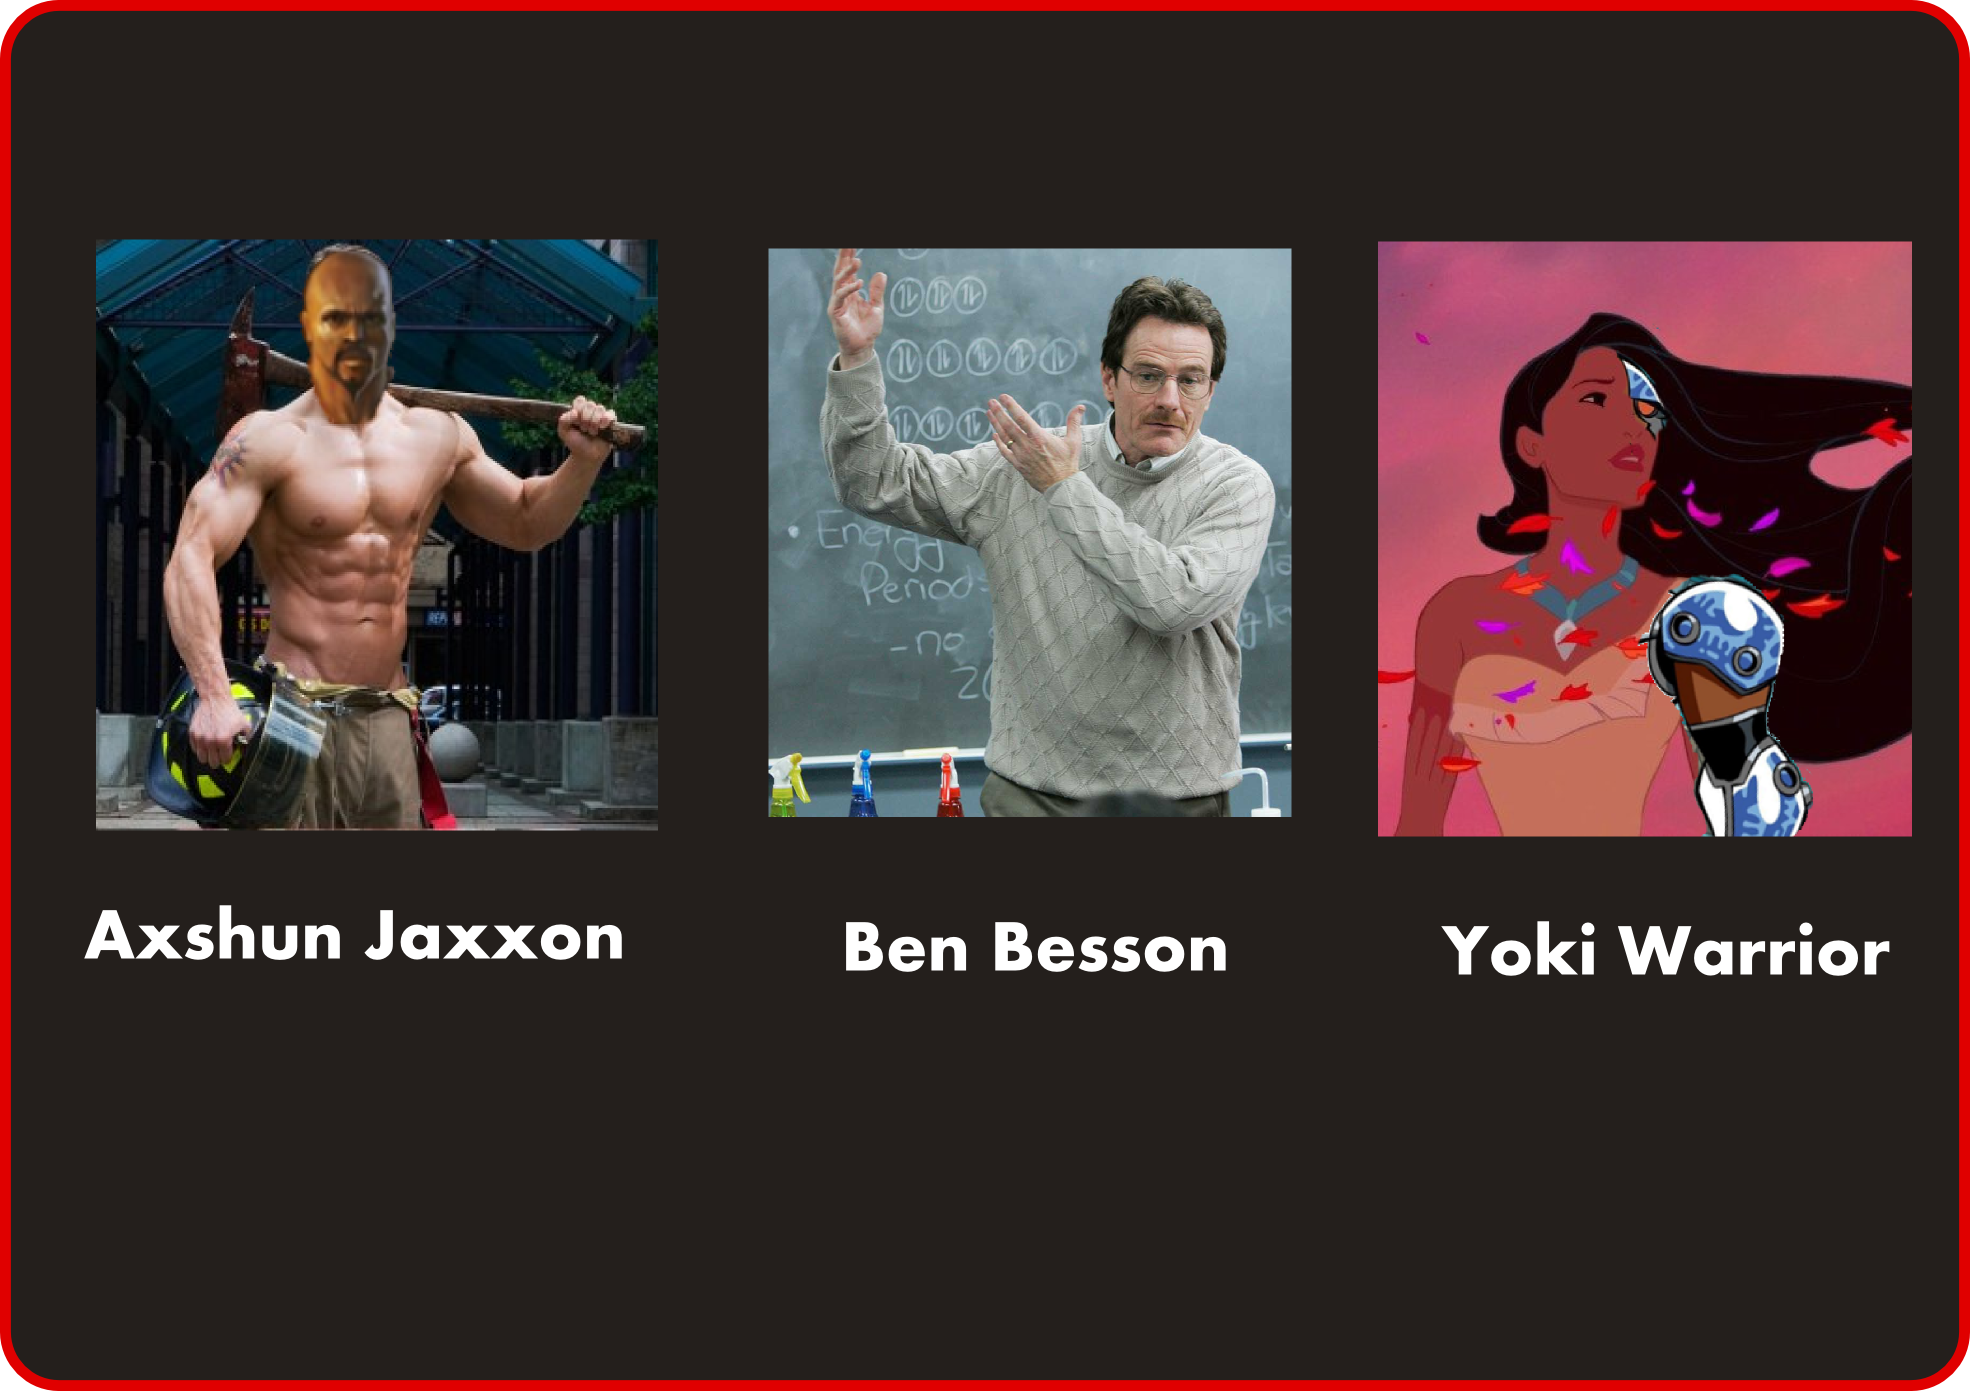
\includegraphics[width=8cm]{./img/character-select.png}
\captionof{figure}{\label{fig:orgcb50883}
Character Select}
\end{center}

\subsubsection{Single Player}
\label{sec:org69ccb77}
The player will load into a room and be alone except for certain gameplay prompts and the occasional message from Mittens. There will be no multiplayer support.

\subsubsection{Introduction}
\label{sec:orgbcbb173}
Upon loading the application, the HoloLens will scan the room and generate scenarios for each of the three characters. The application will not allow players to physically move to different rooms. If the player does, then the application will suspend in a paused state until the player either starts a new game in the new room or returns to the old room.

After the player selects a character, the respective abduction video will play. This will set up the setting of the game and a reason for why the character is trapped in the scenario. When the player awakens in their room, there will be a glowing note. The note will detail the player's goal to solve puzzles and escape the rooms as well as give a hint towards one of the puzzles in the current room.

\begin{enumerate}
\item Axshun Jaxxon
\label{sec:org79550a8}
If the player chooses Axshun Jaxxon, the abduction video will show Axshun Jaxxon's abduction after saving the child from the burning barn.

\item Ben Benson
\label{sec:org238dd2a}
If the player chooses Ben Benson, the abduction video will show Ben Benson's abduction after the lab explosion.

\item Yoki warrior
\label{sec:orga6a54a5}
If the player chooses Yoki Warrior, the abduction video will show Yoki Warrior's abduction after the fight with the cyborg bear.
\end{enumerate}

\subsubsection{Puzzles}
\label{sec:orgd484908}
A puzzle will have interactable 3D objects in the form of holograms. Puzzles will have some random components in order to prevent "trial and error" attempts. Puzzles may or may not be linked to each other where the first puzzle gives a clue to the second puzzle, and the second puzzle will give two answers. The answers will be a number.

\subsubsection{Rooms}
\label{sec:orgc131786}
A room will have four puzzles that spawn randomly within and twelve keys that are marked. Each room will also spawn a random number less than 5 of decoys which will be a misleading clue or a puzzle that will have no usable answer. Each room will have two easy puzzles, one medium puzzle, and one hard puzzle. The four puzzles must be solved in order to get four numbers that represents the four keys to use on four locks. Using the correct keys will unlock the door and allow the player to proceed. After solving a room's puzzles, a checkpoint will will be offered. If the player chooses to take a checkpoint, the game will save and pause for continuation later. If the player forgoes the checkpoint, the game will continue without saving. This mechanic will prevent players from seeing the scenario, leaving, and taking out-of-game time to solve puzzles.

\subsubsection{Scenarios}
\label{sec:orgab7df90}
Each character has a scenario procedurally generated per playthrough. Each scenario has three rooms. Each scenario has a time limit of \textbf{1 hour} to solve all puzzles and escape all three rooms. In order to complete a scenario, every puzzle must be solved within the time limit. For any given room of the scenario, if the player uses an incorrect key set, there will be a \textbf{1 minute penalty}. If the player fails to complete a scenario, a hologram will display a video feed of the expository. 

\subsubsection{Mittens}
\label{sec:orgb49db88}
When the player has been in the game for \textbf{10 minutes}, if a puzzle has not been solved, Mittens will appear to give the player a hint in case they're stuck. This is also when Mittens will introduce himself to the player. During this interaction, time will be paused and puzzles will become uninteractable. If a hint is given, Mittens will disappear and reappar every \textbf{10 minutes} that a puzzle has not been solved to give a new hint. Hints will be consistent for each playthrough of the same scenario.

\subsubsection{Expository}
\label{sec:orgd5a280c}
In each hologram, there will be a model of the character chosen. The character will be shown to meet a gruesome end via randomly generated threats such as cybernetic bears bursting through the walls or the room becoming a trash compactor to squish the player into a cube. If the player completes a scenario within the time limit, a hologram of a Company manager will appear and congratulate the player. The player is then offered a choice to join the Company. If the player joins the company, the character's exposition story plays. If the player refuses, the character's respective world power will have a sleeper agent appear to knock out the manager and help the player character escape. Then, the character will join their respective world power.

\begin{itemize}
\item Axshun Jaxxon will join the Afindican Warlords.

\item Ben Benson will join the Chinese Conglomerate.

\item Yoki Warrior will join the Nomads.
\end{itemize}


\subsection{Hints}
\label{sec:orge3e46b8}
Mittens can give the player several types of hints after the player answers a riddle.
\begin{enumerate}
\item \textbf{Remove Decoys}: Remove all or some of the decoys in the room.
\item \textbf{Puzzle Explanation}: Explain part of a puzzle to make it easier for the player to solve.
\item \textbf{Answer Location}: Place a glow on an object required for a puzzle.
\end{enumerate}

\section{Puzzle Types}
\label{sec:org7e79aea}
\subsection{Acrostic}
\label{sec:org86c6001}
There will be two pages appearing in the room for this puzzle. The first page contains clue phrases that, when answered, provide a mapping of letters to numbers (See Figure \ref{fig:org08c060e}). The second page has a series of blank spaces and numbers (See Figure \ref{fig:org57d90e7}) that make a sentence when the mapping from page 1 is applied (See Figure \ref{fig:org02cfcd5}). The results of this puzzle will be a number for the key or a hint for another puzzle.

\begin{center}
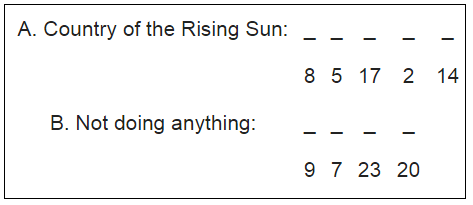
\includegraphics[width=4cm]{./img/acrostic-1.png}
\captionof{figure}{\label{fig:org08c060e}
Page 1}
\end{center}

\begin{center}
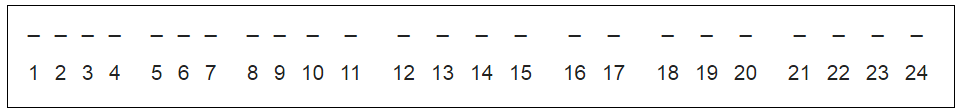
\includegraphics[width=8cm]{./img/acrostic-2.png}
\captionof{figure}{\label{fig:org57d90e7}
Page 2}
\end{center}

\begin{center}
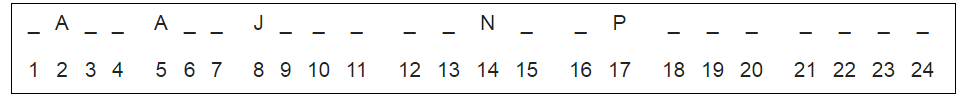
\includegraphics[width=8cm]{./img/acrostic-3.png}
\captionof{figure}{\label{fig:org02cfcd5}
Filling characters in on second page}
\end{center}

\subsection{Rope Chain}
\label{sec:orgc2e7179}
There will be four \textbf{20 foot} ropes each with four pegs spaced at different distances apart attached along the rope. Only one rope will have the exact peg separation required to insert each peg into four anchored podiums across the room.

\begin{center}
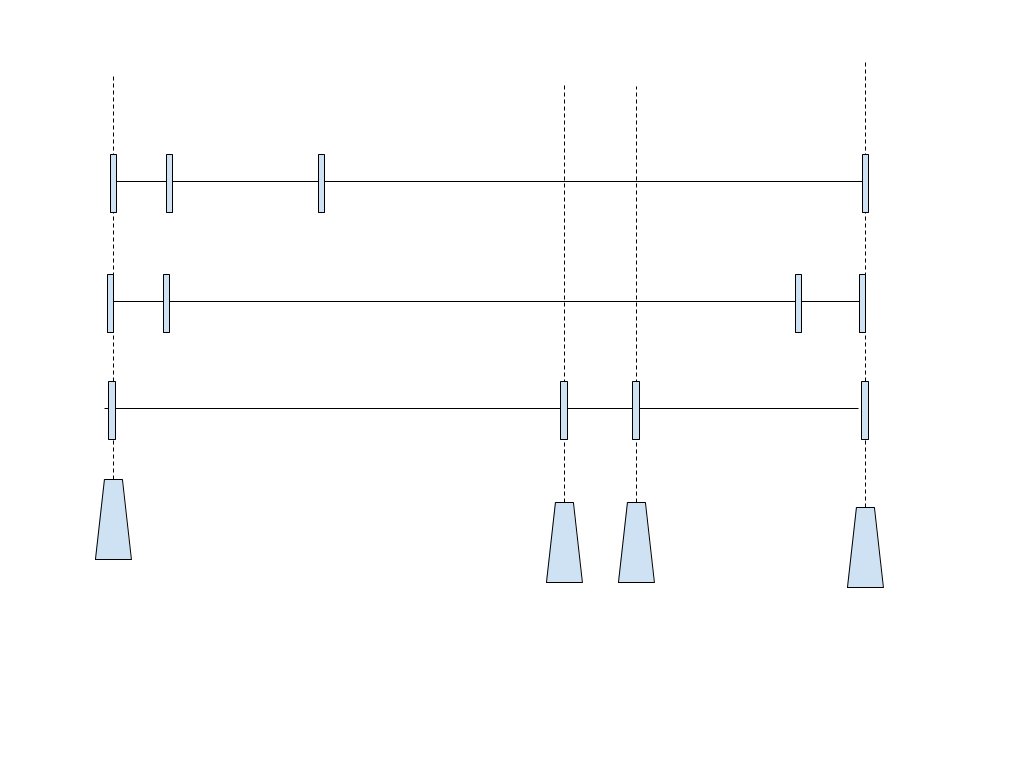
\includegraphics[width=.9\linewidth]{./img/pt-rc-001.png}
\captionof{figure}{\label{fig:orgeb0da18}
An example of the ropes, pegs, and podiums.}
\end{center}

\subsection{Block and Key}
\label{sec:org3423979}

\begin{center}
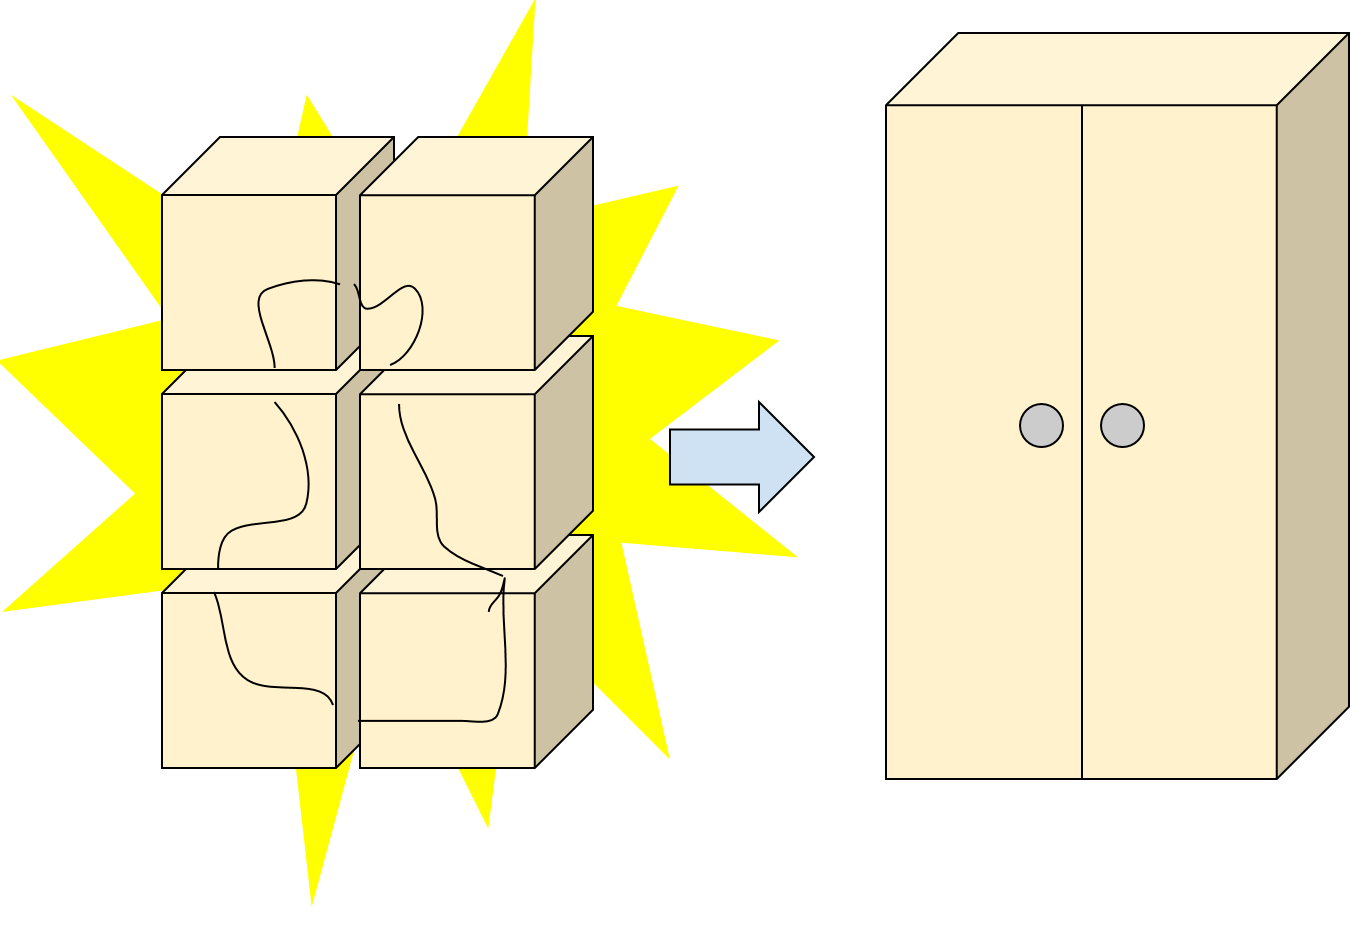
\includegraphics[width=.9\linewidth]{./img/blockandkey.png}
\captionof{figure}{\label{fig:orgeef089a}
Block and key example.}
\end{center}

There will be six \textbf{1 foot} cubes spread across the room. The player will need to place and orient these blocks on a pedestal to create an image by aligning the engravings on each cube. The opposite side of the cube array will then reveal an answer required to escape the room.

\subsection{Cryptogram}
\label{sec:orgc9fa035}

\begin{center}
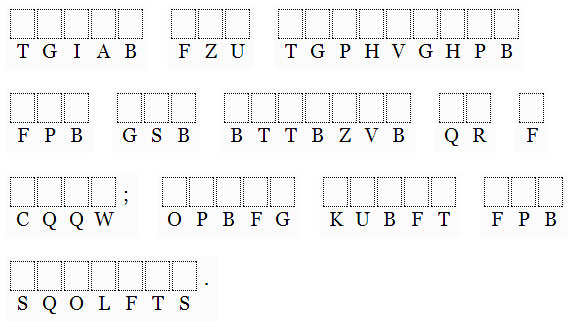
\includegraphics[width=.9\linewidth]{./img/cryptogram.png}
\captionof{figure}{\label{fig:orgca055c5}
Example of a cryptogram.}
\end{center}

A cryptogram is a puzzle that consists of a short piece of encrypted text. Generally the cipher used to encrypt the text is simple enough that that the cryptogram can be solved by hand. Frequently used are substitution ciphers where each letter is replaced by a different letter or number. To solve the puzzle, one must recover the original lettering.

\subsection{Connect the Dots}
\label{sec:org5c84eb1}

\begin{center}
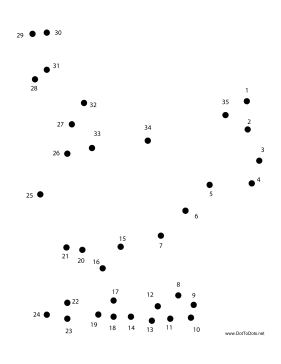
\includegraphics[width=.9\linewidth]{./img/connect.png}
\captionof{figure}{\label{fig:org2c7f841}
Example of a connect the dots.}
\end{center}

Images drawn may be of other objects in the room. Different shaped dots (e.g. square vs. circle) will connect to make different images. A key will be placed in the room to indicate which dots make the correct image.

\subsection{Statues/Totems}
\label{sec:org2ee60f5}

\begin{center}
\includegraphics[width=.9\linewidth]{./img/totem.png}
\captionof{figure}{\label{fig:orge35b92b}
Example of a totem puzzle.}
\end{center}

\textbf{3-4} statues or obelisks with images need to be positioned in a particular way to unlock an answer. There will be an image, that may or may not be the result of the solution of another puzzle, depicting how to orient the statues around the room.

\pagebreak

\section{References}
\label{sec:org34e05b0}
\begin{itemize}
\item \href{https://en.wikipedia.org/wiki/Acrostic\_(puzzle)}{Acrostic} - Wikipedia entry.
\item \href{https://en.wikipedia.org/wiki/Cryptogram}{Cryptogram} - Wikipedia entry.
\item \href{http://www.bloodandbones.com/ph12sim/types.htm}{Puzzle Idea List} - A list of puzzle ideas.
\item \href{http://www.accelerated-ideas.com/news/uncharted-4-chapter-1-2-puzzle-solution-rotating-balls.aspx}{Rotating balls and Symbols} - A description of the rotating balls and symbols puzzle from Uncharted 4.
\item \href{http://www.gameshampoo.com/magazine/articles/24/uncharted-3-all-puzzle-solutions.html}{Uncharted 3 All Puzzles} - All of the puzzles in Uncharted 3.
\item \href{http://www.imgrum.org/media/1023891329744782117\_1530550655}{Axshun Jaxxon} - Axshun Jaxxon's Head.
\item \href{https://s-media-cache-ak0.pinimg.com/originals/14/52/4c/14524cd75630c87f04407c2113094535.jpg}{Axshun Jaxxon} - Axshun Jaxxon's Body.
\item \href{http://www.disneystoryoriginspodcast.com/wp-content/uploads/2013/11/pocahontas1.jpg}{Pocahontas} - Yoki Warrior's Body.
\item \href{http://vignette2.wikia.nocookie.net/teentitans/images/2/2a/Cyborg-teen-titans-9542604-1024-768.jpg/revision/latest?cb=20120115083426}{Cyborg} - Yoki Warrior's Arm and Eye.
\item \href{https://cdn2.content.compendiumblog.com/uploads/user/2c9b66c6-7b80-4006-afb9-8204439bca12/60041788-356f-4b71-b236-b0b9c78f8f0d/Image/dc62e65ec149fb09ea2446f1560db77c/71\_\_of\_earths\_surface\_kevin\_m\_\_gill\_\_flikr.jpg}{Earth} - Base image for Earth.
\item \href{http://img-2.newatlas.com/microsoft-hololens.jpg?auto=format\%2Ccompress\&ch=Width\%2CDPR\&crop=entropy\&fit=crop\&h=347\&q=60\&w=616\&s=63631a238d01aeb6b842d3c31b3898eb}{HoloLens} - Base image for menu selection.
\item \href{https://img.clipartfest.com/b7559eb47d8ee1fe0e3831da8005a24a\_-vehicles-for-businessman-clipart-of-a-businessman-silhouette\_1080-1080.jpeg}{The Company} - The company anonymous figures.
\item \href{https://cdn.dottodots.net/samples/Cat\_7\_Dot-To-Dot.png}{Connect} - Connect the dots.
\item \href{https://gaming.stackexchange.com/questions/34061/whats-the-right-position-of-each-of-the-armors-in-the-chateau}{Totems} - Totem puzzle.
\end{itemize}
\end{document}
